% !TeX program = pdflatex
\documentclass[11pt]{article}
\usepackage[a4paper,margin=25mm]{geometry}
\usepackage[utf8]{inputenc}
\usepackage[T1]{fontenc}
\usepackage{lmodern}
\usepackage{amsmath,amssymb}
\usepackage{booktabs,array,tabularx}
\usepackage{enumitem}
\usepackage{xcolor}
\usepackage{hyperref}
\usepackage{fancyhdr}
\usepackage{tcolorbox}
\usepackage{microtype}
\usepackage{tikz}
\usetikzlibrary{arrows.meta,positioning}

\definecolor{navy}{HTML}{17365D}
\definecolor{blue}{HTML}{2D5ABB}
\definecolor{lightblue}{HTML}{EEF4FB}
\definecolor{warmgray}{HTML}{F5F4F1}
\definecolor{darkgray}{HTML}{444444}
\hypersetup{colorlinks=true,linkcolor=navy,urlcolor=blue,citecolor=navy}
\setlength{\parindent}{0pt}
\setlength{\parskip}{0.55em}
\setlength{\headheight}{14pt}
\setlength{\emergencystretch}{2em}
\setlist{itemsep=0.25em,topsep=0.35em}
\pagestyle{fancy}
\fancyhf{}
\lhead{Engineering Thinking}
\rhead{Lecture Notes}
\cfoot{\thepage}
\renewcommand{\headrulewidth}{0.4pt}
\AddToHook{cmd/section/before}{\clearpage}

\newtcolorbox{keyidea}[1][]{colback=lightblue,colframe=blue,
  boxrule=0.7pt,arc=1.5mm,title={#1},fonttitle=\bfseries}
\newtcolorbox{definition}[1][]{colback=warmgray,colframe=darkgray,
  boxrule=0.6pt,arc=1.5mm,title={#1},fonttitle=\bfseries}
\newtcolorbox{conceptcheck}[1][]{colback=white,colframe=blue,
  boxrule=0.6pt,arc=1.5mm,title={#1},fonttitle=\bfseries}
\newtcolorbox{uncovered}[1][]{colback=white,colframe=darkgray,
  boxrule=0.6pt,arc=1.5mm,title={#1},fonttitle=\bfseries}

\title{\vspace{-2em}\textbf{Lecture 2: Engineering Thinking}}
\author{Dr. Changlai Du}
\date{}

\begin{document}
\maketitle

\begin{keyidea}[Learning goals]
After this lecture, you should be able to formulate an engineering problem before committing to a solution, define observable success criteria, reason about constraints and trade-offs, choose a minimum viable product, decompose a system into responsibilities, and define abstraction boundaries through clear interface promises.
\end{keyidea}

\tableofcontents

\section{Engineering Thinking and the Campus Event Challenge}

Engineering thinking is a disciplined way to frame problems, reason about possible solutions under constraints, and improve those solutions using evidence. Programming is part of this work, but writing code begins only after we understand what the system is meant to accomplish.

The running case study is a campus event-registration service:
\begin{quote}
The university wants an app for students to register for campus events. Your team has one week. Where would you begin?
\end{quote}

The statement already suggests an app, but it does not yet state the underlying problem. Beginning with screens, buttons, or a database risks building a technically functional system that does not address the real need.

\subsection{The problem behind the proposed app}

Before selecting a solution, ask:
\begin{itemize}
  \item Who experiences the problem?
  \item What happens today?
  \item Which assumptions should we check with students and organizers?
  \item Could a simpler process solve the problem without a new app?
\end{itemize}

Students may currently register through group messages or forms while organizers update spreadsheets by hand. Information can become inconsistent: a student may not know whether a place is confirmed, and an organizer may not have an accurate attendance list. A useful working problem statement is therefore:

\begin{definition}[Working problem statement]
Students cannot reliably determine whether they have a confirmed place, and organizers struggle to maintain an accurate attendee list.
\end{definition}

This wording identifies affected users and observable difficulties. ``Build an app'' names a possible solution, not the problem itself. For a small number of events, a shared form, a spreadsheet, and a clear confirmation procedure might be enough. For repeated events with many participants, a dedicated system may be justified. Evidence from the users and the current process should guide that choice.

Each simpler alternative has a cost. A spreadsheet can record registrations, but the organizer must spend considerable time checking submissions, updating rows, resolving duplicates, and keeping the attendee list consistent. A group chat on a third-party instant-messaging service such as WeChat supports communication, but it may not provide the campus identity information required by the registration process. The university's existing campus app already includes a login or user-authentication system, so it can associate an action with a verified campus identity. A third-party messaging account does not necessarily establish who the user is within the university. This difference matters when eligibility and registration rules depend on a student's institutional identity.

Important assumptions include who may register, whether guests are allowed, whether cancellation is possible, how places are confirmed, and whether students actually want another app. Unchecked assumptions often become expensive design mistakes.

\section{Success Criteria, Constraints, and Trade-offs}

\subsection{What counts as success?}

A running program does not by itself establish that a project is finished. The program might implement the wrong policy, lose information, exceed event capacity, or give users an ambiguous result. Success must be stated as an observable outcome for the people who depend on the system.

For the event-registration problem, candidate outcomes include:
\begin{itemize}
  \item a student can find an event and request a place;
  \item the student can clearly tell whether the request was confirmed;
  \item the organizer can obtain an accurate attendee list;
  \item the system never confirms more participants than the event capacity;
  \item a student's confirmed reservation remains available after logging out and returning.
\end{itemize}

These outcomes can become acceptance criteria. For example:
\begin{conceptcheck}[Example acceptance criteria]
\begin{enumerate}
  \item When one place remains and one eligible student registers, the system records exactly one reservation and displays confirmation.
  \item When an event is full, another registration request receives a clear rejection and does not increase the stored attendee count.
\end{enumerate}
\end{conceptcheck}

An acceptance criterion connects a requirement to evidence. We can inspect stored information, run a controlled test, and observe whether a student understands the displayed result.

\subsection{Constraints shape the solution}

The team has one week, four members, limited resources, and limited experience. These constraints make trade-offs unavoidable. Optional features may have to wait, familiar tools may be safer than unfamiliar ones, and the team should protect the correctness of the central registration journey before expanding the product.

One major trade-off concerns user authentication. Implementing a secure login system is complicated. If the university already provides a suitable sign-in service, the team can reuse it rather than rebuild authentication. Reuse does not eliminate responsibility: the team must still check that the component identifies the right users, protects information, and fits the rest of the design.

Trade-offs should not sacrifice the system's essential promise. A small product may omit recommendations or calendar integration, but it must not knowingly overbook events or claim that an unrecorded reservation succeeded.

\section{A Minimum Viable Product}

\begin{definition}[Minimum viable product]
A minimum viable product (MVP) is the smallest usable version that addresses an important user need and lets the team test a meaningful assumption with real users.
\end{definition}

For this case, a complete minimal journey is more useful than several disconnected screens. The first version should allow a student to:
\begin{enumerate}
  \item sign in through an available identity service;
  \item view a list of events and an event's details;
  \item request registration;
  \item receive a clear success or rejection message;
  \item return later and see the registration status.
\end{enumerate}

The organizer should be able to view the resulting attendee list. Behind the interface, the system must remember registrations and enforce the applicable rules, including eligibility and event capacity.

Features that can wait include localization, categories and filters, bookmarking events of interest, social sharing, recommendations, calendar integration, reminders, and an automated waitlist. These ideas may be valuable, but they are not necessary to test whether students can register and understand the outcome.

Letting students try the MVP provides evidence about the design. We can observe whether the registration button is easy to find, whether the confirmation is understandable, and whether a user who returns later can find the recorded status. Feedback can also reveal missing rules or assumptions. A successful database update is not enough if the user cannot tell what happened.

\section{Decomposing the Registration System}

\begin{definition}[Decomposition]
Decomposition divides a problem into smaller responsibilities whose inputs, outputs, and connections can be explained clearly.
\end{definition}

The classroom discussion identified three main parts:
\begin{enumerate}
  \item the front end, which displays events, accepts user actions, and shows results;
  \item the registration logic, which applies the registration rules;
  \item storage, which remembers events, users, and reservations.
\end{enumerate}

Authentication supports the journey by supplying a user identity, but it can be an existing university service rather than a newly implemented subsystem.

\begin{figure}[htbp]
  \centering
  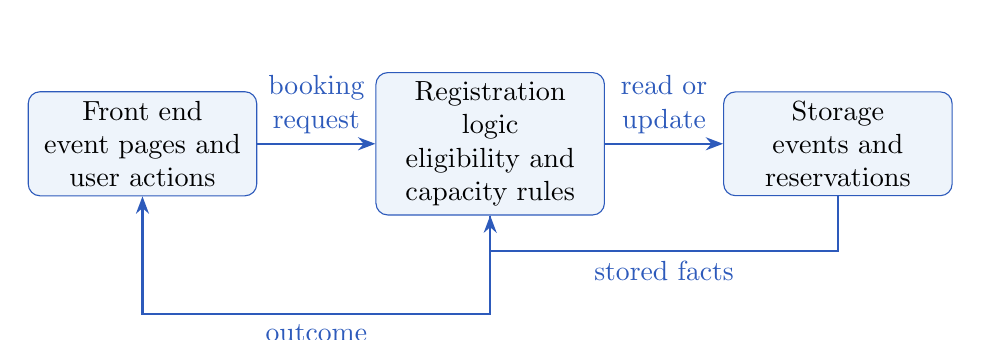
\begin{tikzpicture}[
    part/.style={draw=blue,fill=lightblue,rounded corners=1.5mm,
      minimum height=13mm,text width=0.22\linewidth,align=center},
    flow/.style={-{Stealth[length=2.2mm]},thick,blue},
    node distance=15mm
  ]
    \node[part] (front) {Front end\\event pages and user actions};
    \node[part,right=of front] (logic) {Registration logic\\eligibility and capacity rules};
    \node[part,right=of logic] (store) {Storage\\events and reservations};
    \draw[flow] (front) -- node[above,align=center]{booking\\request} (logic);
    \draw[flow] (logic) -- node[above,align=center]{read or\\update} (store);
    \draw[flow] (store.south) -- ++(0,-0.7) -| node[pos=0.25,below,align=center]{stored facts} (logic.south);
    \draw[flow] (logic.south) -- ++(0,-1.25) -| node[pos=0.25,below,align=center]{outcome} (front.south);
  \end{tikzpicture}
  \caption{A responsibility-level decomposition of the event-registration system.}
  \label{fig:registration-decomposition}
\end{figure}

\subsection{Inputs and outputs}

The front end receives user input and event information. A registration action produces a request containing at least the user's identity and the event's identity. The front end later displays the outcome returned by the registration logic.

The registration logic receives the request and the facts needed to evaluate it. It checks rules such as:
\begin{itemize}
  \item whether the user is eligible for the event;
  \item whether guests are allowed;
  \item whether registration is still open;
  \item whether the event has remaining capacity;
  \item whether the user already has a reservation.
\end{itemize}

If the request is allowed, the logic sends an authorized update to storage. Storage accepts queries and updates, remembers the reservation, and later returns stored facts. The logic then reports a confirmed reservation, a rule-based rejection, or a system error.

\subsection{How the parts complete one registration}

One possible interaction is:
\begin{enumerate}
  \item The student selects an event and clicks the registration button.
  \item The front end sends the student identity and event identity to the registration logic.
  \item The registration logic obtains the relevant event and reservation state.
  \item The logic applies the rules.
  \item If the request is permitted, storage records the reservation.
  \item Only after successful storage does the system return confirmation for the front end to display.
\end{enumerate}

The three parts can each appear to work independently while the whole system fails. For example, the logic may produce correct information in a format that storage does not accept. The page may interpret ``request received'' as ``reservation confirmed.'' The components therefore need agreed interfaces and shared meanings, not merely individually correct code.

\section{Abstraction and the Boundary Between Parts}

\begin{definition}[Abstraction]
Abstraction exposes the behavior that another part needs while hiding implementation details that the caller does not need.
\end{definition}

The event page does not need to know how reservations are stored. The storage might use a relational database, a spreadsheet, or a text file. The page also does not need to know the database table layout or the internal steps used to check capacity. It needs a clear way to request a reservation and interpret the result.

The same separation works in the other direction. The back end does not need to know whether the registration button appears near the top or bottom of the page, whether ten or twenty events appear at once, or which colors the page uses to distinguish an interesting event from a confirmed registration.

\subsection{A precise interface promise}

\begin{keyidea}[Contract for \emph{reserve a place}]
Given a valid student identity and event identity, the operation returns \emph{confirmed} only when the registration satisfies the rules and a durable reservation has been stored. Otherwise, it returns a clear rejection or error without claiming that registration succeeded.
\end{keyidea}

The word \emph{confirmed} has a shared meaning across the boundary. It is not merely an acknowledgement that a click or request reached the server. It means that the rules passed and the system remembers the reservation.

With this contract, the team can change the internal storage method without changing the event page, provided the interface and promised behavior remain the same. The abstraction makes independent change possible, but it does not excuse incorrect implementation. Every implementation behind the boundary must still keep the promise.

\section{Questions Reserved for the Next Lecture}

The class did not reach the remaining material in the slide deck. The following pages therefore preserve the questions only. No speaker-note answers are included.

\subsection{Modules and reuse}
\begin{uncovered}[Build or reuse?]
Which parts should we build ourselves, and which could we reuse?
\end{uncovered}
\begin{uncovered}[Modules and reuse]
\begin{itemize}
  \item If the booking policy changes, which part should change?
  \item Could an existing sign-in component meet our needs?
  \item What must we check before depending on a reused component?
\end{itemize}
\end{uncovered}

\subsection{A shared development process}
\begin{uncovered}[Team development]
How can four people turn these parts into one reliable app?
\end{uncovered}
\begin{uncovered}[Shared process]
\begin{itemize}
  \item How do we know which version to use?
  \item What should a teammate check before accepting a change?
  \item What does ``done'' mean for a feature and for the whole app?
\end{itemize}
\end{uncovered}

\subsection{A double-booking failure}
\begin{uncovered}[Competing requests]
What if two students try to book the last place at the same time?
\end{uncovered}
\begin{uncovered}[One place, two requests]
A checks availability. One place remains.\\
B checks availability. One place remains.\\
A receives confirmation.\\
B receives confirmation.

Each request followed the usual steps. Why did the system fail?
\end{uncovered}
\begin{uncovered}[A symptom and a broken rule]
\begin{itemize}
  \item What rule must always remain true?
  \item Which observation shows that the rule has failed?
  \item What do we know so far, and what are we only guessing?
\end{itemize}
\end{uncovered}

\subsection{Debugging with evidence}
\begin{uncovered}[Finding the cause]
How would you find the cause of the double-booking bug?
\end{uncovered}
\begin{uncovered}[Evidence from the investigation]
One request at a time works. Two overlapping requests can fail. The logs show that both requests read ``1 place left'' before either saves.
\begin{itemize}
  \item What hypothesis fits this evidence?
  \item What experiment would test it?
\end{itemize}
\end{uncovered}
\begin{uncovered}[A fix we can explain]
\begin{itemize}
  \item What is the smallest change that addresses the cause?
  \item How would we check that the fix works and does not break other behavior?
  \item Which test should we keep so the bug does not return?
\end{itemize}
\end{uncovered}

\subsection{Testing, validation, and iteration}
\begin{uncovered}[Readiness]
What evidence would convince you that the app is ready for real users?
\end{uncovered}
\begin{uncovered}[Correct behavior and useful outcomes]
\begin{itemize}
  \item Which failure would you test first?
  \item Could all our tests pass while students still find the app confusing?
  \item How do testing and debugging help us in different ways?
\end{itemize}
\end{uncovered}
\begin{uncovered}[The next version]
What should we change after students try the first version?
\end{uncovered}
\begin{uncovered}[Feedback and responsibility]
\begin{itemize}
  \item What did the feedback reveal about our original assumptions?
  \item If AI proposes the change, what must we still check?
  \item How would we know that the new version is better?
\end{itemize}
\end{uncovered}

\subsection{Synthesis}
\begin{uncovered}[Engineering thinking]
Which kinds of thinking did we use besides writing code?
\end{uncovered}
\begin{uncovered}[Your explanation]
\begin{itemize}
  \item How would you explain engineering thinking to a friend?
  \item Which question will you ask before your next team project?
\end{itemize}
\end{uncovered}

\section{Optional Transfer Questions}

These extension questions also appeared after the lecture material and were not discussed in class.
\begin{uncovered}[Campus equipment loan service]
How would you apply the same thinking to a campus equipment loan service?
\end{uncovered}
\begin{uncovered}[A short engineering proposal]
\begin{itemize}
  \item State the problem and one constraint.
  \item Choose a useful first version.
  \item Identify the responsibilities and one component you might reuse.
  \item Propose a failure test.
  \item Explain how you would investigate a failure.
\end{itemize}
\end{uncovered}

\section*{Homework}
\addcontentsline{toc}{section}{Homework}
Read the assigned material on \emph{Version Control}. Review both the material from Lecture 1 and the engineering-thinking questions from this lecture in preparation for the next quiz.

\section*{Sources Used for These Notes}
\addcontentsline{toc}{section}{Sources Used for These Notes}
These notes synthesize the slide deck \emph{02 Engineering Thinking.pptx}, its embedded speaker notes for the portion presented in class, and the classroom transcript dated 13 October 2026. The transcript begins after the opening portion because screen recording was not started at the beginning. Slides 1--6 were therefore reconstructed from the deck. The transcript and deck jointly support the detailed notes for slides 7--12. For slides 13 onward, only the questions shown on the slides have been reproduced; answers from the speaker notes have intentionally been omitted.

\end{document}
